% SPAR Final Report — Temporal Awareness in LLMs
% To compile: latexmk -pdf report.tex

\documentclass[final]{sparreport}

\title{Probing and Steering Temporal Representations in LLMs for AI Oversight}

\author{
  \textbf{Justin Shenk}\\
  \texttt{shenk.justin@gmail.com}\\
  Independent Researcher
  \and
  Jyotin Goel,
  Tejas Bijoor,
  Michal Mraz,
  Vansh Gupta,
  Ipshita Das,\\
  Ronen Eldan,
  Harleen Bagga,
  Avigya Paudel,
  Archit Sharma,\\
  Tim Obiso,
  Adrian Molofsky,
  Joseph Rudoler
}

\sparround{Spring 2026}

\begin{document}

\maketitle

% ============================================================================
% ABSTRACT
% ============================================================================
\begin{abstract}
We investigate how large language models internally represent and process temporal information, an open question with direct implications for AI safety --- particularly for understanding planning capability, deception detection, and oversight robustness. Across 11 complementary sub-projects, we apply linear probes, causal interventions (activation steering), and behavioral evaluations to models ranging from 1B to 30B parameters. Our findings show that temporal representations are genuinely encoded in LLM activations and can be causally steered, but that careful baselines are essential: in code generation, what appears to be planning signal is fully explained by surface features. We also find safety-relevant phenomena including context fatigue (entropy collapse over long contexts), sycophantic surrender under social pressure, and a tentative link between short-term temporal steering and more harmful outputs. These results motivate both methodological caution in probing studies and further investigation of temporal representations as a lever for AI safety monitoring.
\end{abstract}

\keywords{mechanistic interpretability \and temporal reasoning \and linear probes \and activation steering \and AI safety}

% ============================================================================
% INTRODUCTION
% ============================================================================
\section{Introduction}

Understanding how LLMs represent time internally is relevant to several AI safety concerns. Models that encode temporal horizons may develop planning capabilities, and the ability to detect and steer these representations could inform oversight mechanisms \cite{li2023inference, rimsky2024steering}. If a model distinguishes short-term from long-term reasoning, this distinction may also relate to deceptive alignment \cite{hubinger2019risks} --- where a model behaves differently based on perceived temporal context such as training versus deployment \cite{park2023ai}.

This project brings together 11 researchers investigating complementary facets of temporal representation in LLMs. Sub-projects span probing for temporal structure in activations, causal steering of temporal horizons, evaluating lookahead planning in code generation, measuring context fatigue over long sequences, detecting sycophantic surrender under social pressure, tracking uncertainty encoding across reasoning steps, and analyzing activation stability under repetition.

Our shared codebase\footnote{\url{https://github.com/justinshenk/temporal-awareness}} and common methodological toolkit --- linear probes on residual stream activations, activation steering via probe-derived directions, and behavioral evaluations --- enable cross-model and cross-task comparisons that no single sub-project could achieve alone.

Success for this project means producing publishable findings on how temporal information is encoded and used in LLMs, developing reusable methodology for probing studies (including rigorous baseline protocols), and identifying safety-relevant properties of temporal representations that could inform runtime monitoring. Figure~\ref{fig:structure} illustrates the research structure across the three layers of analysis.

\begin{figure}[htbp]
  \centering
  \includegraphics[width=\textwidth]{figures/diagram4-stack.png}
  \caption{Research structure of the Temporal Activation Monitors project. The bottom layer shows the models under study (1B--30B parameters). The middle layer maps probing and steering contributions across fellows. The top layer shows safety-relevant applications that build on the probing results.}
  \label{fig:structure}
\end{figure}

% ============================================================================
% METHODOLOGY
% ============================================================================
\section{Methodology}

\subsection{Common Framework}

All sub-projects share a core methodology: train linear probes on transformer residual stream activations to detect temporal features \cite{belinkov2022probing}, then validate with causal interventions. We extract activations at each layer from frozen pretrained models and train logistic regression or linear classifiers to predict temporal properties (e.g., short-term vs.\ long-term horizon, temporal order, uncertainty level). Where probes detect signal, we perform activation steering by adding scaled probe directions to residual streams during generation \cite{li2023inference} and measuring behavioral change.

\subsection{Models}

We evaluate models across four architecture families and a range of scales: GPT-2 (124M--1.5B), Pythia (410M--2.8B), Qwen3 (4B, 8B, 30B-A3B MoE), Llama-3.2 (1B, 3B), Phi-3-mini-4k, CodeLlama-7B, and SantaCoder. This breadth allows us to test whether findings generalize across architectures and whether scale thresholds exist for specific capabilities.

\subsection{Datasets and Evaluation}

Each sub-project constructs task-specific evaluation sets, with contrastive pair datasets following the Contrastive Activation Addition (CAA) framework \cite{rimsky2024steering}. Notable datasets include: 1,000 validated implicit temporal pairs across 40 categories and 8 domains, with no explicit temporal keywords (Paudel); code generation samples with 500 examples across 5 return types for the planning study (Bijoor); sycophancy benchmarks with social pressure conditions (Bagga); and repetition-degradation benchmarks across 4 datasets with 10 repetition counts (Molofsky). We use bootstrap resampling (typically 1,000 iterations) for statistical significance testing and PCA for dimensionality reduction where applicable.

\subsection{Methodological Innovations}

Three innovations emerged from the sub-projects. First, a \textbf{baseline staircase protocol} (Bijoor): chance $\to$ bag-of-words $\to$ name-only $\to$ name+params $\to$ probe, which progressively tests whether probe accuracy reflects genuine internal computation or surface features. Second, \textbf{pooled-activation probes} (Mraz): aggregating across token positions rather than using only the last token, yielding improved probe performance. Third, \textbf{implicit temporal pairs} (Paudel): evaluation data that tests temporal reasoning without temporal keywords, preventing probes from relying on lexical shortcuts.

% ============================================================================
% RESULTS
% ============================================================================
\section{Results}

\subsection{Temporal Representations Are Real and Steerable}

Linear probes across Qwen3-4B, Llama-3.2-3B, and Phi-3-mini confirm that temporal and process-state information is genuinely encoded in LLM activations \cite{tenney2019bert}. Paudel achieves 99.2\% probe accuracy at layer 26 of Qwen3-4B for classifying short-term vs.\ long-term thinking on implicit pairs (no temporal keywords), with shuffled-label controls at chance. Steering works best at layers 19--22 (not the probe's best layer), with layer 22 at $\alpha = 50$ yielding approximately $4\times$ more probability on long-term completions. Interactive results are available online.\footnote{Paudel: \url{https://avi161.github.io/temp-steering-results/}; Paudel slides: \url{https://docs.google.com/presentation/d/10pftLZsDfvfAfPHRN3k_f5jSffTAO_5SYrJj2QAULkI/}}

\begin{figure}[htbp]
  \centering
  \includegraphics[width=0.85\textwidth]{figures/temporal-steering-dashboard.png}
  \caption{Temporal orientation steering sweep (Paudel). Layer-by-layer and alpha-by-alpha results from 702 manually scored responses, showing best long-term config (+6.8, layer 20, $\alpha$=50) and best short-term config ($-$2.3, layer 18, $\alpha$=50).}
  \label{fig:steering-paudel}
\end{figure}

Obiso finds that temporal computation is causally localized to the last three layers (29--31) of Qwen3-4B via causal patching \cite{meng2022locating}, and that probe accuracy updates token-by-token during autoregressive generation --- an ``internal clock'' that tracks temporal context in real time. The linear component of temporal representations transfers across domains, while the nonlinear component is domain-specific, supporting linear probes as the appropriate tool for universal temporal monitoring.

Sharma confirms temporal representations exist across all three models tested but vary in robustness: Qwen3 shows the most distributed and robust signal, Llama exhibits strong but less clean generalization, and Phi displays weaker, more localized behavior.

\begin{figure}[htbp]
  \centering
  \includegraphics[width=0.95\textwidth]{figures/papers/paudel-fig1.png}
  \caption{Temporal preference concepts (Paudel). \emph{Top-left:} localization --- probe accuracy across layers. \emph{Top-right:} geometry of temporal-preference activations colored by horizon, from seconds to centuries. \emph{Bottom:} steering effect across layers 19--22.}
  \label{fig:paudel-fig1}
\end{figure}

\subsection{Baselines Matter: Deflating Apparent Planning Signal}

Bijoor's investigation of lookahead planning in code generation provides a cautionary result. Across all 11 models tested (GPT-2 family, Pythia 410M--2.8B, SantaCoder, CodeLlama-7B, Llama-3.2-1B), initial probing suggested 80--91\% accuracy at predicting return types --- apparently strong evidence of planning. However, the baseline staircase reveals this is fully explained by surface features: a name+params baseline (a classifier trained on function name and parameter names alone) achieves 87--95\% accuracy, consistently beating the probe ($p \approx 1.0$ across every model and layer). Misleading-name experiments confirm models follow parameter names 56\% of the time and function names 22--34\%. Generation-time probing shows probe accuracy actually \emph{decays} during generation, and acrostic behavioral tests (4--20\%, near chance) confirm these models cannot perform structural planning. This frames as a methodology contribution: a ``baseline staircase'' protocol for deflating spurious probing results.

\begin{figure}[htbp]
  \centering
  \includegraphics[width=0.85\textwidth]{figures/papers/bijoor-fig1.png}
  \caption{Baseline staircase result (Bijoor). The name+params baseline matches or exceeds the residual-stream probe across all 11 models tested, deflating the apparent planning signal.}
  \label{fig:baseline-staircase}
\end{figure}

\subsection{Safety-Relevant Phenomena}

\textbf{Sycophancy.} Bagga finds that social pressure causes answer flip rates of 10--62.5\%, but true sycophantic surrender occurs in only 1.5--15.5\% of cases. Output confidence is an unreliable safety monitor: 23.4\% of high-confidence correct answers still surrendered under pressure, including some at confidence 1.0. Hidden-state signal for predicting surrender emerges only in the final layer quartile, but the critical probe remains underpowered (11 positive examples; $\sim$1,000 needed).

\textbf{Context fatigue.} Eldan demonstrates that entropy collapse is a real problem as context fills, with models growing more confident without corresponding accuracy gains. This is partially counteracted by in-context learning, where models sometimes improve at a task pattern over the context window.

\textbf{Uncertainty encoding.} Das finds that uncertainty is strongly encoded at the first reasoning step but weakens after subsequent reasoning, is distributed across layers, and only weakly predicts future states. Across datasets, uncertainty encoding varies significantly and consistently degrades from step 1 to step 2.

\textbf{Steering and safety.} Obiso observes that steering toward long-term thinking monotonically increases output safety, while short-term steering produces more violent completions --- a finding that, if confirmed, would link temporal horizon representations directly to safety-relevant behavior. Additionally, smaller models (4B) show stronger deception detection than larger ones (9B), suggesting internal ``honesty'' may degrade with scale.

\subsection{Emerging Directions}

Goel is developing an analysis of token trajectories for multihop questions, with an initial outline established. Gupta is investigating phase transitions in temporal horizon representations, aiming to establish how models transition from short-horizon to long-horizon reasoning and identify features that support each. Molofsky has completed Phase 1 behavioral experiments (8 models $\times$ 4 datasets $\times$ 10 repetition counts) with Phase 2 targeting sparse autoencoders \cite{cunningham2023sparse}, finding that patience degradation is model- and task-specific: Llama-3.1-8B shows clear accuracy degradation on temporal reasoning (TRAM), Qwen3-8B shows a warm-up effect, and Qwen3-30B-A3B (MoE) remains stable.

\begin{figure}[htbp]
  \centering
  \includegraphics[width=0.85\textwidth]{figures/papers/goel-fig1.png}
  \caption{Knowing-saying gap methodology overview (Goel). A pipeline that contrasts clean and corrupted-prior variants of $\sim$500 multi-hop math problems, then fits a probe to residual-stream activations, with the probe firing at $p > 0.64$ as a real-time signal for intervention.}
  \label{fig:goel}
\end{figure}

\begin{figure}[htbp]
  \centering
  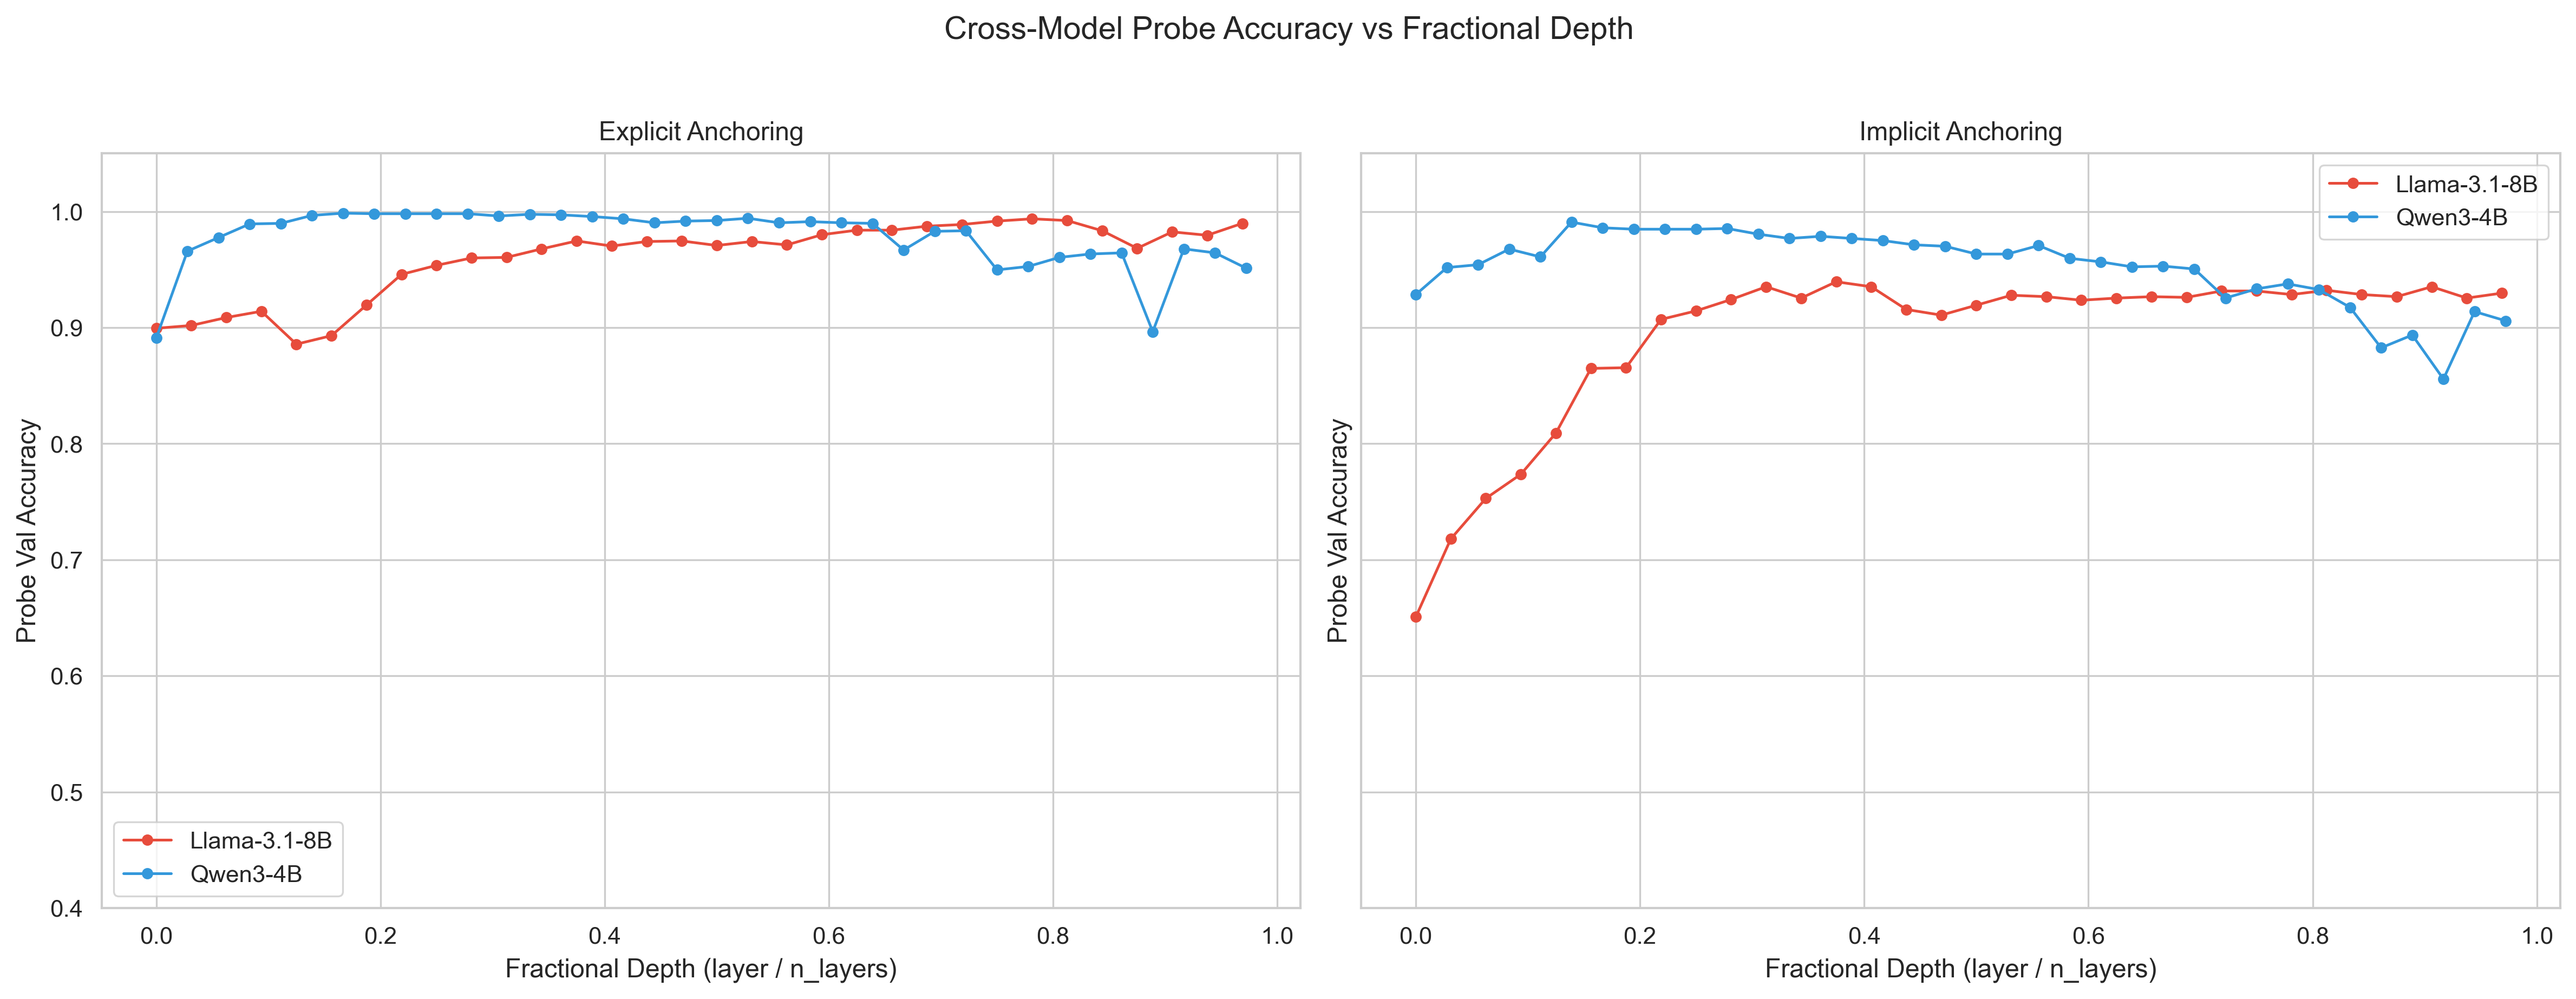
\includegraphics[width=0.95\textwidth]{figures/papers/vansh-figure.png}
  \caption{Cross-model probe accuracy vs.\ fractional depth (Gupta), comparing Llama-3.1-8B and Qwen3-4B. \emph{Left:} explicit anchoring; \emph{right:} implicit anchoring. Qwen3-4B reaches near-ceiling accuracy by $\sim$0.2 of depth in both regimes, while Llama-3.1-8B ramps up more gradually under implicit anchoring before catching up at deeper layers.}
  \label{fig:gupta}
\end{figure}

% ============================================================================
% FELLOW SUMMARY
% ============================================================================
\section*{Fellow Summary}

\begin{table}[htbp]
\centering
\small
\begin{tabular}{p{2.2cm}p{4.5cm}p{4.5cm}p{2cm}}
\toprule
\textbf{Fellow} & \textbf{Research Question} & \textbf{Key Finding} & \textbf{Target} \\
\midrule
Jyotin Goel & Token trajectories for multihop reasoning & Initial outline on trajectory analysis & Publication \\
Tejas Bijoor & Lookahead planning in code generation & No planning found; baseline staircase deflates all signal & Publication \\
Michal Mraz & Improved probe training for temporal features & Pooled probes outperform last-token; causal steering confirmed & Publication \\
Vansh Gupta & Phase transitions in temporal horizon & Establishing short-to-long horizon transition & Publication \\
Ipshita Das & Uncertainty encoding across reasoning steps & Uncertainty strong at step 1, degrades after reasoning & Publication \\
Ronen Eldan & Context fatigue in long contexts & Entropy collapse is real; partially offset by ICL & Publication \\
Harleen Bagga & Sycophancy detection via hidden states & Sycophancy in 1.5--15.5\% of cases under social pressure; confidence unreliable as monitor & Publication \\
Avigya Paudel & Temporal steering on implicit pairs & 99.2\% probe accuracy; $4\times$ steering effect at layer 22 & Pub + Demo \\
Archit Sharma & Cross-model temporal representation comparison & Signal varies: Qwen robust, Phi weak, Llama intermediate & Publication \\
Tim Obiso & Causal localization of temporal computation & Last 3 layers; linear component transfers cross-domain & Publication \\
Adrian Molofsky & Patience degradation under repetition & Degradation is model- and task-specific; SAE phase next & Publication \\
\bottomrule
\end{tabular}
\caption{Summary of fellow research questions, key findings, and target outputs.}
\label{tab:fellows}
\end{table}

% ============================================================================
% CHALLENGES & OPEN QUESTIONS
% ============================================================================
\section{Challenges \& Open Questions}

\textbf{Scale limitations.} The absence of lookahead planning across all models up to 7B parameters raises the question of whether genuine structural planning requires significantly larger models (70B+), where chain-of-thought reasoning capabilities emerge. Testing at this scale would require additional compute resources.

\textbf{Statistical power.} Several sub-projects face sample size constraints. The sycophancy probe (Bagga) has only 11 positive examples for the critical hidden-state prediction task and needs approximately 1,000 to be conclusive. Scaling these experiments is a priority for follow-on work.

\textbf{Linear vs.\ nonlinear representations.} Obiso's finding that linear probe components transfer across domains while nonlinear components are domain-specific raises interpretive questions: are we capturing the safety-relevant signal with linear probes, or missing critical nonlinear structure?

\textbf{Surface cue confounds.} The baseline staircase result (Bijoor) demonstrates that probe accuracy can be entirely explained by surface features. This motivates broader adoption of rigorous baselines across all probing sub-projects and careful evaluation of whether temporal probes in other contexts might face similar confounds.

% ============================================================================
% FUTURE WORK
% ============================================================================
\section{Future Work}

Several threads extend beyond the SPAR program and remain open for follow-on work:

\begin{enumerate}
  \item \textbf{Scale underpowered experiments}: expand the sycophancy dataset (Bagga) to $\sim$1,000 positive examples to properly power the hidden-state prediction probe. Complete Phase 2 (activation probes + SAEs) of the patience-degradation study (Molofsky) across the remaining models, targeting precursor gap detection.

  \item \textbf{Test generalization}: 1,000 validated implicit temporal pairs across 40 categories (Paudel) remain available as a clean held-out set. Cross-model causal-patching analysis (Sharma) is the natural next step for determining whether temporal representations are functionally equivalent across architectures.

  \item \textbf{Confirm steering--safety link}: Obiso's observation that short-term steering increases violent completions requires systematic confirmation with larger sample sizes and controlled generation.

  \item \textbf{New directions}: extend the phase-transition hypothesis for temporal horizon representations (Gupta), complete the token-trajectory analysis for multihop reasoning (Goel), and further characterize the interaction between context fatigue and in-context learning (Eldan).

  \item \textbf{Publication targets}: the baseline staircase methodology (Bijoor) and temporal steering results (Obiso, Paudel) are the most publication-ready outputs. Sub-projects are being prepared for ICML 2026 workshops, with several also targeting COLM 2026; supporting blog posts and web demos cover preliminary and negative findings.
\end{enumerate}

% ============================================================================
% REFERENCES
% ============================================================================
\bibliographystyle{plain}
\bibliography{references}

\end{document}
